\documentclass[border=0.5cm]{standalone}
\usepackage{tikz}
\usepackage{tikzlings-penguins}
 
\begin{document}
 
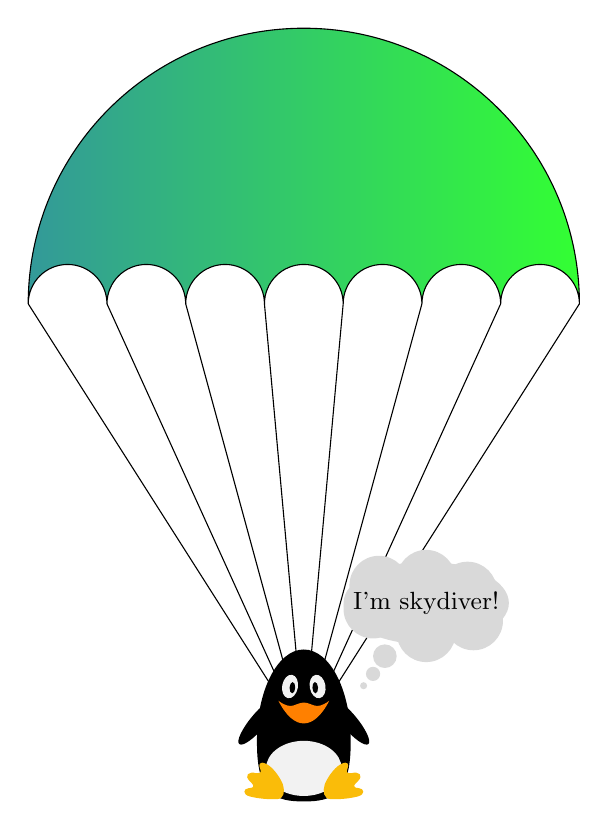
\begin{tikzpicture}
 
% Canopy
\draw[left color=teal!80,right color=green!80](0:3.5) arc(0:180:3.5)  
\foreach \i in {1,...,7}{arc (180:0:0.5) }-- cycle;
 
% Suspension lines
\foreach \i in {-3.5,...,3.5} 
{
\draw (\i,0) -- (0,-5.5);
}
 
% Skydiver (Penguin)
\begin{scope}[yshift=-6.5cm]
\penguin
\thing[
    think={\small I'm skydiver!},
    scale=1.5,
    yshift =-0.6cm,
    xshift=-0.05cm]
\end{scope}
 
\end{tikzpicture}
 
\end{document}